%!TEX root = ../Studienarbeit.tex

\chapter{Validierung und Gegenüberstellung}

\todo[inline]{Ab hier überarbeiten}

\section{Validierung des Funktionsumfangs}

In diesen Abschnitt der Studienarbeit befindet sich der Vergleich des definierten Aufgabenumfangs von Kapitel \ref{section:Aufgabenstellung} zu dem realisierten Funktionsumfang. Falls Einschränkungen im realisierten Funktionsumfang vorhanden sind, werden diese erläutert.

\subsection{Softwareentwicklung}
Alle Anforderungen zur Software des Erweiterungsmoduls sind in Kapitel \ref{section:softwareRequirement} definiert. Die erste definierte Anforderung ist, die Unterstützung von verschiedenen Betriebssystemen am Endgerät für die Übermittlung von Fernsteuerungsdaten. Die unterstützten Betriebssysteme sollten Android, Windows, Linux und iOS/iPadOS sein. Getestet wurde der Datenaustausch zwischen dem Erweiterungsmodul und den genannten Betriebssystemen, jeweils mit einer Betriebssystemversion und einer Simulatorsoftware. Android wurde in der Version 10 mit der Simulatorsoftware \textit{FPV.SkyDive} getestet und der vollständige Funktionsumfang konnte nachgewiesen werden. Unter Windows 11 mit der Simulatorsoftware \textit{Velocidrone} konnte ebenso der vollständige Funktionsumfang des Erweiterungsmoduls nachgewiesen werden. Als Linux-Betriebssystem wurde \textit{Pop! OS 22.04 LTS} mit der Simulatorsoftware \textit{Velocidrone} verwendet. Dort konnte gleichermaßen der vollständige Funktionsumfang nachgewiesen werden. Für die Überprüfung des Funktionsumfangs des Erweiterungsmoduls mit iOS/iPadOS 16.3.1 wurde die Simulatorsoftware \textit{FPV.SkyDive} verwendet. Dort konnte nur eine eingeschränkte Funktionsfähigkeit nachgewiesen werden. Zum einen findet der Verbindungsaufbau zwischen dem Erweiterungsmodul und dem iOS/iPadOS-Endgerät statt. Zum anderen werden vom Erweiterungsmodul übermittelten Daten mit dem iOS/iPadOS-Endgerät empfangen. Nachgewiesen werden kann dies mit der Software \textit{packetLogger} und \textit{libimobiledevice}, womit alle \ac{HCI}-Nachrichten des iOS/iPadOS-Endgeräts betrachtet werden können. Für weitere Betrachtungen wurde ein, mit iOS/iPadOS kompatibler, Nintendo Switch-Controller verwendet und der Kommunikationsaustausch zwischen dem iOS/iPadOS-Endgerät und dem Nintendo Switch-Controller betrachtet. Dabei stellt sich heraus, dass der Nintendo Switch-Controller mittels \ac{BBR} die Gamecontrollerdaten übertragt. Wie in Quelle \cite{lemmingDevESP32Comment} beschrieben ist, müssen \ac{BLE}-Gamecontroller durch das \ac{MFi}-Programm zertifiziert werden und ein zusätzliches Hardwaremodul enthalten, entgegen der ursprünglichen Annahme, welche in Kapitel \ref{section:appleAnforderungen} beschrieben ist.

Die zweite Softwareanforderung ist, dass die Kommunikation zwischen dem Erweiterungsmodul und den Endgeräten mittels \ac{BLE} erfolgen und sich das Erweiterungsmodul als \ac{HID}-Gerät authentifizieren soll. Die Umsetzung dieser Anforderung ist in Kapitel \ref{section:bluetoothStackSelection} und \ref{section:communicationModuleDevice} beschrieben.

Die dritte Anforderung ist, dass die Kommunikation zwischen dem Erweiterungsmodul und der Multikopterfernsteuerung über den Modulschacht der Fernsteuerung erfolgen soll. Auch soll die Kommunikation mittels eines vorhandenen Protokolls der Fernsteuerungsfirmware OpenTX oder einer Abspaltung davon erfolgen. Als Kommunikationsprotokoll zwischen dem Erweiterungsmodul und der Multikopterfernsteuerung wird CRSF verwendet, wie in Kapitel \ref{section:communicationCRSF} nachgelesen werden kann. Getestet wurde die Erweiterungsmodulsoftware mit der Multikopterfernsteuerung \textit{Tango 2} von dem Unternehmen \textit{Team Blacksheep} mit der Firmware \textit{FreedomTX} Version \textit{TBS-1.3.0}. Dabei konnten alle von der Fernsteuerung mittels dem CRSF-Protokoll versendeten Kanaldaten von dem Erweiterungsmodul empfangen und verarbeitet werden.

Die vierte Anforderung ist, dass es verschiedene Ein- und Ausgabemöglichkeiten geben soll, damit Endanwender mit dem Erweiterungsmodul interagieren können. Dafür findet einerseits die Ausgabe von Statusnachrichten mittels eines \acs{OLED}-Displays statt, nachzulesen in Kapitel \ref{section:oledOutput}. Andererseits gibt es mehrere Taster für Eingaben durch den Endanwender, nachzulesen in Kapitel \ref{section:softwareCombination}. Ebenfalls war ein Bestandteil dieser Anforderung, dass weitere Statusindikatoren mittels \acp{LED} integriert werden sollen. Dies ist jedoch nicht umgesetzt worden, da alle wichtigen Statusnachrichten für den Endanwender durch das \acs{OLED}-Display angezeigt werden. Lediglich eine Status-\ac{LED} ist vorhanden, um anzuzeigen, ob eine funktionierende Stromzufuhr zum Erweiterungsmodul vorhanden ist. Dies ist jedoch komplett in Hardware realisiert wie in Abbildung \ref{fig:spannungsRegulierung} zu sehen ist.

Die letzte Softwareanforderung ist, dass der Akkustand der Multikopterfernsteuerung an ein verbundenes Endgerät übermittelt wird. Die Softwarekomponente hierfür ist vollständig vorhanden und funktionsfähig, jedoch bietet der Lite-Modulschachtstecker keinen Pin an, an dem die rohe Akkuspannung anliegt (zu sehen in Abbildung \ref{fig:pinoutController}). Aus diesem Grund wird im \ac{BLE}-Akkustand-Merkmal der \ac{HOGP}-Daten immer der Wert 0 übertragen. Hiermit wird sichergestellt, dass der Endanwender des Erweiterungsmoduls selbst den aktuellen Akkustand der Multikopterfernsteuerung überprüfen muss, da der Endanwender davon ausgehen muss, dass das Erweiterungsmodul nicht den korrekten Akkustand übermittelt.

\subsection{Platinenentwurf}
Die Anforderungen an die entworfenen Platinen des Erweiterungsmoduls sind in Kapitel \ref{section:pcbRequirement} aufgelistet. Dabei ist die Hauptanforderung, dass die Erweiterungsmodulplatine alle benötigten Elektronikkomponenten, welche im prototypischen Steckbrettaufbau vorhanden sind, enthalten muss. Zusätzlich sollte die Platine möglichst kompakt sein, damit die Platine an der Multikopterfernsteuerung verwendet werden kann, ohne dass das Erweiterungsmodul während der Verwendung der Fernsteuerung stört. Diese Anforderungen wurden in den Platinen, welche in Kapitel \ref{section:pcbImplementation} vorgestellt wurden, umgesetzt. Die Platine enthält dafür den ESP32-Mikrocontroller, die benötigte Spannungsregulierung für alle Elektronikkomponenten sowie mehrere Taster, ein Display und eine Status-\ac{LED} für die Interaktion mit dem Endanwender. Zusätzlich ist ein \ac{ESD}-Schutz an der Erweiterungsmodulbuchse integriert, ebenso wie weitere Elektronikkomponenten für die komfortablere Programmierung des ESP32-Mikrocontrollers.

\subsection{Gehäuseerstellung}
Die Anforderungen an das Erweiterungsmodulgehäuse sind in Kapitel \ref{section:caseRequirement} aufgelistet und umfassen den Entwurf eines Kunststoffgehäuses, welches für Modulschächte des Typs \textit{Lite} ist und möglichst ohne Nachbearbeitung verwendet werden kann. All diese Anforderungen sind im entworfenen Gehäuse von Kapitel \ref{section:caseImplementation} realisiert worden. Das entworfene Gehäuse ist für Erweiterungsmodulschächte des Typs \textit{Lite} und kann mit vier Stützstrukturen gedruckt werden. Da diese an nicht sichtbaren Stellen des Gehäuses gedruckt werden, entfällt die Nachbearbeitung der Oberflächen an diesen Stellen.

\section{Gegenüberstellung \acs{BLE}-Modul und USB-Verbindung}
Ein wichtiges Merkmal von Fernsteuerung sowohl während der Trainings im Simulator als auch während des Fliegens mit realen Multikoptern, ist die Latenz zwischen der Eingabe an der Fernsteuerung bis zur Verarbeitung an der Gegenstelle. Um diese Latenz zu bestimmen werden im nachfolgenden Abschnitt mögliche Versuchsaufbauten verglichen und  die Ergebnisse des präferierten Versuchsaufbaus ausgewertet. Die ausgewerteten Ergebnisse werden ebenso mit weiteren Computereingabegeräten verglichen.

\subsection{Versuchsaufbauten}
Zur Bestimmung der Latenz der Fernsteuerung muss ein Versuchsaufbau erstellt werden, mit welchen sowohl der Zeitpunkt der Tastenbetätigung als auch der Zeitpunkt des Eingabeereignisses im Betriebssystem gemessen werden kann. Zusätzlich sollte der Versuchsaufbau ohne Änderungen an der vorhandenen Multikopterfernsteuerung funktionieren.

Ein Versuchsaufbau der ohne Änderung an der Multikopterfernsteuerung auskommt ist, dass mittels eines Computerprogramms eine Person aufgefordert wird eine bestimmte Taste an der Fernsteuerung schnellstmöglich zu bestimmten Zeitpunkten zu bestätigen. Im Hintergrund wird durch das Computerprogramm die Zeit zwischen der Aufforderung und dem Zeitpunkt des Eingabeereignisses gemessen. Dieses Verfahren hat jedoch den Nachteil, dass in jeder Messung noch die Reaktionszeit der Person inbegriffen ist und in jedem Durchlauf unterschiedlich sein kann. Dadurch sind die Testergebnisse nicht repräsentativ, weshalb dieser Ansatz nicht weiter verfolgt.

Ein weiteres Verfahren, welches ohne Veränderungen an der Multikopterfernsteuerung auskommt, ist eine angepasste Version des vorhergehenden Ansatzes. Dabei wird der Tastendruck von einer Person, durch einen Tastendruck mittels eines Servos ausgetauscht. Der Servomotor kann dabei eigenständig durch das Computerprogramm angesteuert werden. Zur Befestigung des Servomotors an der Fernsteuerung muss zusätzlich eine Stützstruktur entwickelt werden, womit der Servomotor bei jedem Versuchsdurchlauf an der optimalen Position über dem Taster liegt. Zu sehen ist dieser Versuchsaufbau in Abbildung \ref{fig:servoTestStation}. Die Latenz in diesem Verfahren kann dadurch bestimmt werden, indem zunächst der Zeitpunkt für den Befehl des Tastenloslassens von dem Servomotor protokolliert wird. Im darauffolgenden Schritt muss noch der Zeitpunkt des Eingabeereignisses ermittelt werden und die Differenz beider Zeitpunkte stellt dabei die Latenz dar. Die Latenz in diesem Verfahren bei dem die Multikopterfernsteuerung mittels USB mit dem Testrechner verbunden ist, beträgt zirka 100~ms. Jedoch weicht die Latenz dieses Verfahren weit von den Ergebnissen der Arbeit, welche in Quelle \cite{wimmerLatenzStation} zu finden sind und realistische Werte bilden, ab. Diese Abweichung kommt zustande, da der Zeitpunkt des Tastenloslassens nur zu Beginn der Servomotorbewegung bestimmt werden kann und dadurch die Bewegungszeit des Servomotors in jeder Messung mit inbegriffen ist. Deshalb wird dieses Versuchsverfahren ebenso nicht verwendet.

\begin{figure}[H]
    \centering
    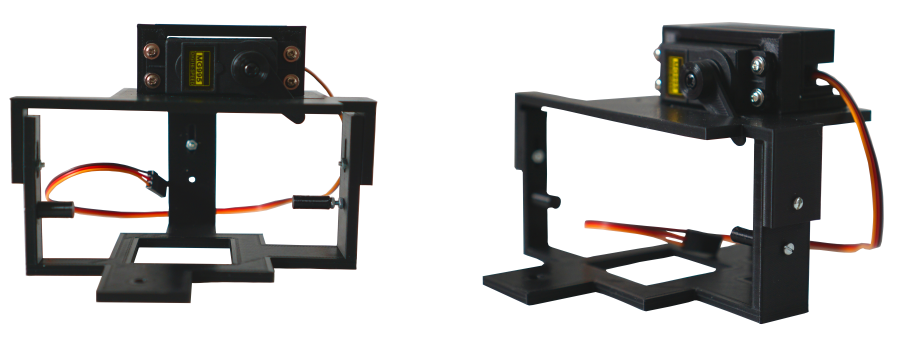
\includegraphics[width=.6\textwidth]{servoTestStation}
    \caption{Stützstruktur für einen Versuchsaufbau zum Betätigen eines Fernsteuerungstasters mittels eines Servos}
    \label{fig:servoTestStation}
\end{figure}

Für den verwendeten Versuchsaufbau wird als Grundlage, das Versuchsverfahren aus der Arbeit in Quelle \cite{wimmerLatenzStation} verwendet. Dieses Verfahren setzt jedoch voraus, dass Veränderungen an der Multikopterfernsteuerung durchgeführt werden. Die Betätigung des Tasters der Fernsteuerung findet hierbei mittels eines Optokopplers statt, wodurch an dem Fernsteuerungstaster zwei Kabel angelötet werden müssen.

Ein Optokoppler ist eine Elektronikkomponente mit welcher Signale galvanisch getrennt übertragen werden können \cite{elektronikKompendiumOptokoppler}. Das zu übertragende Signal wird dabei mittels einer \ac{LED} -- als Sendeelement -- und einer Fotodiode -- als Empfangselement -- übertragen. Zu sehen ist das zugehörige Ersatzschaltbild eines Optokopplers in Abbildung \ref{fig:optocoupler}.

\begin{figure}[H]
    \centering
    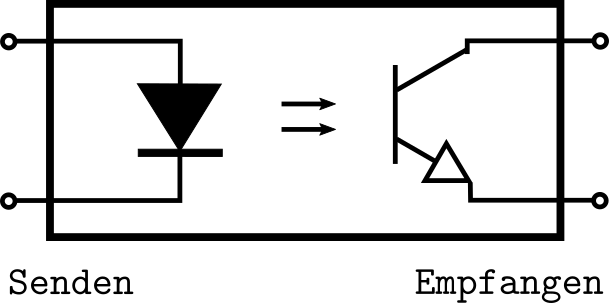
\includegraphics[width=.3\textwidth]{optocoupler}
    \caption{Ersatzschaltbild eines Optokopplers; abgewandelt von \cite{altiumOptokoppler}}
    \label{fig:optocoupler}
\end{figure}

Für die Ausführung der Latenzmesssoftware wird der Einplatinencomputer Raspberry Pi Model B+ verwendet. Dieser bietet ansteuerbare \acs{GPIO}, womit die \ac{LED} des Optokopplers geschaltet wird. Betrieben wird der Einplatinencomputer mit dem Betriebssystem \textit{Raspbian GNU/Linux 11 (bullseye)} und dem Linux-Kernel Version \textit{5.15.61+}. Zur Auswertung der Eingabeereignisse im Linux-Kernel wird die Schnittstelle evdev, welche in Kapitel \ref{section:evdevExplained} beschrieben ist, verwendet. evdev kann sowohl für die Auswertung von \ac{BLE}- als auch USB-Eingabeereignisse verwendet werden. Als Latenz in diesem Versuchsaufbau wird die Zeit zwischen dem Deaktivieren der \ac{LED} des Optokopplers und dem Auftreten des Eingabeereignisses im Kernel des Einplatinencomputers verwendet. Der zugehörige Versuchsschaltplan ist in Abbildung \ref{fig:optoTestStation} zu sehen.

\begin{figure}[H]
    \centering
    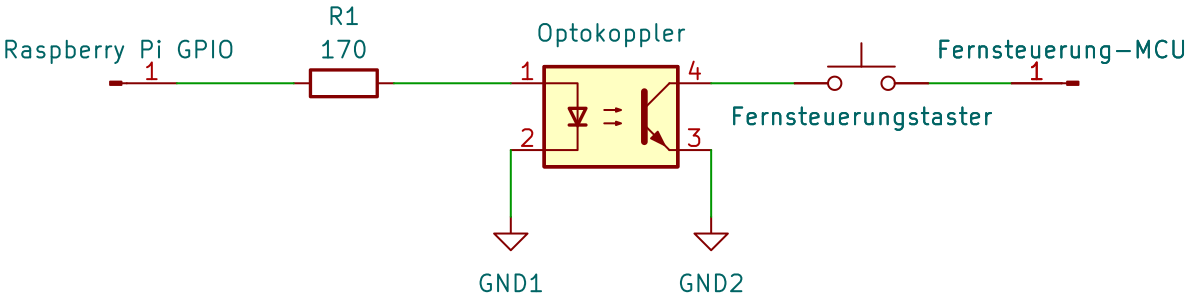
\includegraphics[width=.8\textwidth]{optoTestStation}
    \caption{Schaltplan des Versuchsaufbaus zur Bestimmung der Latenz mittels eines Optokopplers; abgewandelt von \cites{wimmerLatenzStation}[S.~8; S.~12]{LTV817}}
    \label{fig:optoTestStation}
\end{figure}

\subsection{Auswertung}
Sowohl für die Auswertung der USB-Latenz als auch für die Auswertung der \ac{BLE}-Latenz erfolgten jeweils 5000 Versuchsdurchläufe. Die Versuchsergebnisse werden dabei als Schwarmplot dargestellt, indem jede Messung als eigenständiger Punkt dargestellt wird \cite[S.~7]{wimmerLatenzStation}. Dadurch können die Versuchsergebnisse dieser Arbeit gut mit den Ergebnissen aus Quelle \cite{wimmerLatenzStation} verglichen werden, da dort die Ergebnisse im selben Format bereitgestellt werden. 

\subsubsection{USB-Latenz}
In Abbildung \ref{fig:latencyUSBAll} sind alle 5000 Durchläufe des Versuchsdurchlaufs als Schwarmplot dargestellt. Während des Versuchsdurchlaufs wurden alle 5000 Tastenbefehle an der Fernsteuerung durch den Einplatinencomputer als Eingabeereignis erkannt. Der Latenzmittelwert aller Durchläufe liegt bei 9,16~ms und die Standardabweichung bei 2,26~ms. Durch diese Ergebnisse befindet sich die Latenz mittels der USB-Verbindung der Multikopterfernsteuerung im Vergleich zu den getesteten Eingabegeräten von Quelle \cite{wimmerLatenzStation} zu den 50~\% mit einer geringeren Latenz.

\begin{figure}[H]
    \centering
    \includegraphics[width=.7\textwidth]{latencyUSBAll}
    \caption{Latenz aller Versuchsdurchläufe mittels USB-Verbindung}
    \label{fig:latencyUSBAll}
\end{figure}

\subsubsection{\ac{BLE}-Latenz}
Von allen 5000 Versuchsdurchläufen mittels der \ac{BLE}-Verbindung konnten am Einplatinencomputer sieben Eingabeereignisse nicht erkannt werden. Von allen erkannten Durchläufen lag dabei der Latenzmittelwert bei 52,22~ms und die Standardabweichung bei 97,32~ms. Die Standardabweichung ist deshalb groß, da wie in Abbildung \ref{fig:latencyBLEAll} zu sehen ist 267 Messergebnisse außerhalb von 100~ms liegen und dadurch der Versuchsergebnisbereich eine große Spreizung aufweist. Werden jedoch die Messergebnisse größer 100~ms herausgerechnet liegt der Latenzmittelwert bei 30,00~ms und die Standardabweichung bei 7,68~ms, wie in Abbildung \ref{fig:latencyBLElt100} zu sehen ist. In nachfolgenden Kapitel ist beschrieben, warum Messergebnisse größer 100~ms in der Praxis vernachlässigt werden können. Jedoch gehört in beiden Fällen die \ac{BLE}-Verbindung des Fernsteuerungserweiterungsmoduls im Vergleich zu den Eingabegeräten der Quelle \cite{wimmerLatenzStation} zu den Eingabegeräten mit der größten Latenz.

\begin{figure}[H]
    \centering
    \includegraphics[width=.7\textwidth]{latencyBLEAll}
    \caption{Latenz aller Versuchsdurchläufe mittels \ac{BLE}-Verbindung}
    \label{fig:latencyBLEAll}
\end{figure}

\begin{figure}[H]
    \centering
    \includegraphics[width=.7\textwidth]{latencyBLElt100}
    \caption{Latenz aller Versuchsdurchläufe die kleiner 100~ms sind mittels \ac{BLE}-Verbindung}
    \label{fig:latencyBLElt100}
\end{figure}

\subsubsection{Ergebniserläuterung}
\label{section:resultExplanation}
Zu Erkennen ist sowohl in dem USB- als auch in dem \ac{BLE}-Schwarmplot, dass es bestimmte Regionen gibt, an denen sich die Messergebnisse häufen. Dies liegt bei der USB-Verbindung daran, dass Eingabedaten durch das Endgerät in bestimmten Intervallen abgefragt werden und keine Daten ausgehend vom Eingabegerät versendet werden können \cites[S.~48f., S.~277ff.]{usb2Spec}[S.~5]{wimmerLatenzStation}. Dies ist unter einer \ac{BLE}-Verbindung nicht der Fall, da Werteänderungen eines Eingabegerätes an abonnierte Endgeräte durch das Eingabegerät selbständig verschickt werden \cite[S.~1516]{bluetoothCore}. Die größere Latenz durch das Erweiterungsmodul mit der \ac{BLE}-Verbindung hat drei Gründe. Der erste Grund ist, dass mehrfache Umwandlung zwischen unterschiedlichen Protokollen stattfinden muss bis die Fernsteuerungsbefehle am Endgerät ankommen. Zunächst müssen die Steuerungsdaten in der Fernsteuerung in CRSF-Pakete umgewandelt werden. Darauf folgend müssen diese Pakete im Erweiterungsmodul in BLE-Pakete umgewandelt werden, bevor diese vom Endgerät ausgewertet werden können. Hingegen müssen bei der USB-Übertragung nur die Steuerungsdaten in ein USB-Paket umgewandelt werden. Als zweiter Grund ist zu nennen, dass nicht jedes CRSF-Paket, welches über den Modulschacht verschickt wird, Steuerungsdaten enthält, sondern wie in Kapitel \ref{section:crsfProtocol} beschrieben auch weitere Statusinformationen enthalten kann. Dadurch entsteht in diesem Schritt eine Latenz welche ein Vielfaches von 6~ms ist. Als letzter Grund ist noch zu nennen, dass das \ac{BLE}-Übertragungsintervall zwischen dem Erweiterungsmodul und dem Endgerät dynamisch verhandelt werden kann. Dabei kann ein Gerät eine Anfrage zur Änderung der Verbindungsparameter an die Gegenstelle schicken und diese erwidert oder lehnt die Änderung ab. Dabei liegt das Intervall für den minimalen Datenaustausch bei 7,6~ms. In der Erweiterungsmodulsoftware ist dieser minimale Intervallwert auf 11,25~ms gelegt, da dies der Grenzwert bei Apple-Produkten ist, welcher aber nicht von jedem Endgerät angenommen werden muss \cite[S.~188]{appleDesignGuide}. \cite{bleConnectionParameter}

In der Praxis sollten Latenzen über 100~ms und nicht versende Eingabeereignisse mittels dem \ac{BLE}-Erweiterungsmodul seltener auftreten als wie im vorhandenen Versuchsaufbau. Dies hat den Grund, dass im Versuchsaufbau nur immer eine spezielle Taste der Multikopterfernsteuerung betätigt wurde, was jedoch in der Realität nicht vorkommt. Denn während der Verwendung des Erweiterungsmoduls durch einen Multikopterpiloten müssen ständig mehrere Eingabeereignisse nahezu simultan stattfinden, um den Multikopter in der gewünschten Flugbahn zu manövrieren. Daraus folgernd wird sehr häufig veranlasst, dass ein \ac{BLE}-Paket verschickt werden muss, welche alle aktuellen Eingabedaten der Multikopterfernsteuerung enthält.

Durch die zusätzliche Latenz von 20,84~ms (Optimalfall) der \ac{BLE}-Verbindung im Vergleich zur USB-Verbindung würde eine zusätzliche Distanz von ungefähr 0,75~m zurückgelegt, wenn eine Multikoptergeschwindigkeit von 130~km/h angenommen wird \cites{droneSpeed1}{droneSpeed2}{droneSpeed3}. Hierbei muss jedoch mit einbezogen werden, dass es sich zwischen zwei gesendeten Eingabesignalen nicht, um binäre Wertänderungen, sondern meist um kontinuierliche minimale Anpassungen an den Steuerknüppeln handelt, wodurch es nur zu relativen Änderungen in der Flugbahn kommt. Zusätzlich finden große Änderungen der Steuerknüppelpositionen meist nicht bei hohen Geschwindigkeiten statt. Auch können sich Multikopterpiloten in gewisser Weise auf die vorhandene Latenz des Eingabegeräts anpassen und dadurch die gewünschten Steuersignale nach kurzer Eingewöhnungsphase früher einleiten.

Zuletzt ist noch festzuhalten, dass die Testperson (Hobbydrohnenpilot) keinen merkbaren Unterschied zwischen der Steuerung des Simulators mittels der USB- und der \ac{BLE}-Verbindung feststellen konnte.